\documentclass[11pt]{article}
\usepackage[T1]{fontenc}
\usepackage{lmodern}
\usepackage{comment}
\usepackage{fancyvrb}
\usepackage{graphicx}
\usepackage{geometry}
\usepackage{relsize}

% We will generate all images so they have a width \maxwidth. This means
% that they will get their normal width if they fit onto the page, but
% are scaled down if they would overflow the margins.

\makeatletter
\def\maxwidth{\ifdim\Gin@nat@width>\linewidth\linewidth
\else\Gin@nat@width\fi}
\makeatother
\let\Oldincludegraphics\includegraphics
\renewcommand{\includegraphics}[1]{\Oldincludegraphics[width=\maxwidth]{#1}}
\ifxetex
  \usepackage[setpagesize=false, % page size defined by xetex
              unicode=false, % unicode breaks when used with xetex
              xetex]{hyperref}
\else
  \usepackage[unicode=true]{hyperref}
\fi
\hypersetup{breaklinks=true,
            pdfauthor={},
            pdftitle={Refactoring Hello World Application using Dependency Injection},
            colorlinks=true,
            urlcolor=blue,
            linkcolor=magenta,
            pdfborder={0 0 0}}
%\urlstyle{same}  % don't use monospace font for urls
\setlength{\parindent}{0pt}
\setlength{\parskip}{6pt plus 2pt minus 1pt}
\setlength{\emergencystretch}{3em}  % prevent overfull lines
%\setcounter{secnumdepth}{0}

\geometry{
  %includeheadfoot,
  margin=2.54cm
}

\fvset{fontsize=\relsize{0.5}}
\fvset{tabsize=2}

\title{Worksheet: Refactoring a Hello World application using Dependency Injection}

\author{based on a presentation by Sang Shin ex-Sun Java Evangelist}
\date{}

\begin{document}
\maketitle

This worksheet explores the ideas of dependency injection and the Spring framework by exploring
step-by-step refactoring processes for a standard \texttt{Hello World} application.

\section*{Lab Exercises}

\begin{enumerate}
\item Import all the sample code for this lab
\item Build and Run \verb!HelloWorld! sample application
\item Build and Run \verb!HelloWorldWithCommandLineArguments! sample application
\item Build and Run \verb!HelloWorldDecoupled! sample application
\item Build and Run \verb!HelloWorldDecoupledInterface! sample application 
\item Build and Run \verb!HelloWorldDecoupledInterfaceWithFactory! sample application 
\item Build and Run \verb!HelloWorldSpring! sample application
\item Build and Run \verb!HelloWorldSpringWithDI! sample application
\item Build and Run \verb!HelloWorldSpringWithDIXMLFile! sample application
\item Build and Run \verb!HelloWorldSpringWithDIXMLFileConstructorArgument!
\item Build and Run \verb!HelloWorldSpringWithAnnotation! sample application
\item Build and Run \verb!HelloWorldSpringWithAutoscan! sample application
\end{enumerate}

Some of the images are taken from an Eclipse project but the equivalent can be easily 
achieved in IntelliJ or Netbeans.

\section{Download the source code repository}

\begin{enumerate}
\item 
Download the repository which includes the examples for this worksheet.
The relevant code will be under the folders \verb!di! and \verb!springdi!.
\item
Create a new project called \verb!helloworld! (or
whatever name of your choice). As there are several versions of the code 
it is worth spending time organising the code into sub-projects (modules).
\end{enumerate}

\section{Build and Run \texttt{HelloWorld} sample application}

In this exercise, you are going to build the good old \texttt{HelloWorld}
application you probably wrote as your first Java application many years ago\ldots

\begin{enumerate}
\item As most IDEs perform \emph{incremental compilation} there is no need for 
a separate compilation step.

\item Run the application.

%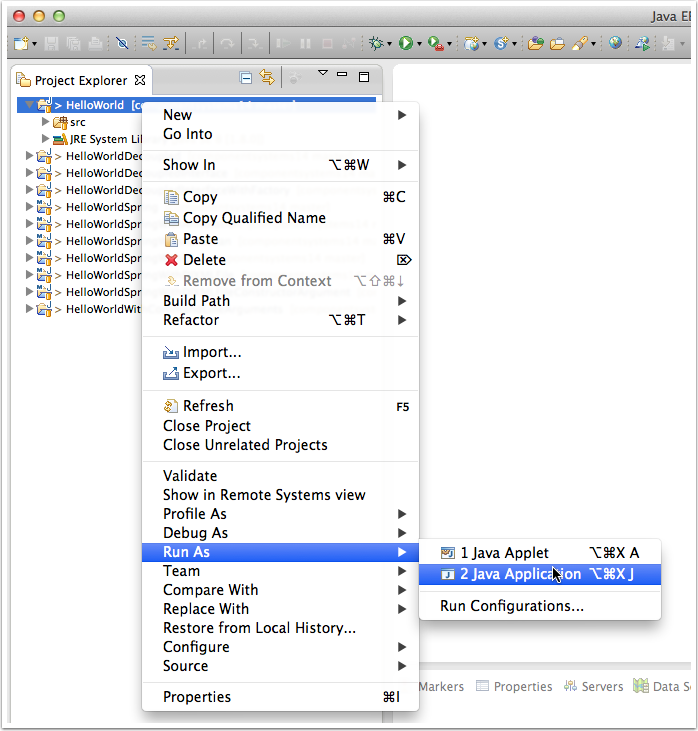
\includegraphics{images/Run-As.png}

\item Observe the result. 

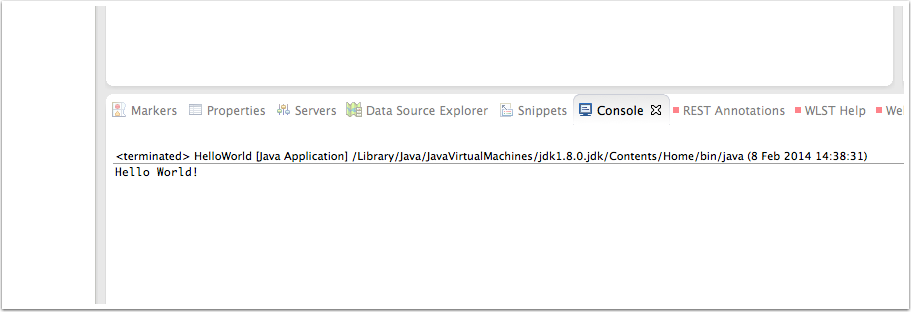
\includegraphics{images/HelloWorld-output.png}

\item Open and study \texttt{HelloWorld.java}.

\begin{itemize}
\item
  Expand \texttt{HelloWorld-\textgreater{}src} (or whatever the project is called).
\item
  Expand \texttt{helloworld}
\item
  Double-click \texttt{HelloWorld.java}.
\end{itemize}
\bigskip

\VerbatimInput[frame=single,label=\fbox{\Large\emph{HelloWorld.java}}]{../../code/HelloWorld/src/helloworld/HelloWorld.java}
\end{enumerate}

\section{Build and Run \texttt{HelloWorldWithCommandLineArguments} sample application}

This code externalises the message content and read it in at runtime,
from the command line argument.
Now you can change the message without
changing and recompiling the code.
\begin{enumerate}
\item Study \texttt{HelloWorldWithCommandLineArguments.java}

\VerbatimInput[frame=single]{../../code/HelloWorldWithCommandLineArguments/src/helloworld/HelloWorldWithCommandLineArguments.java}

\item Run the application.

\item Observe that the text is displayed in the Console.

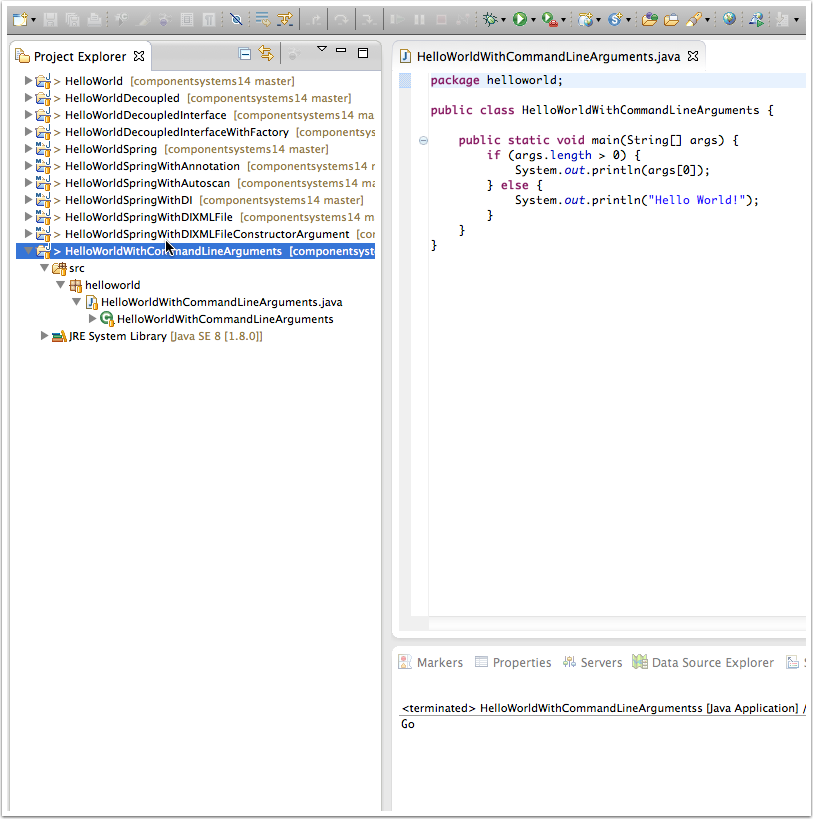
\includegraphics{images/HWCommand-result.png}

\end{enumerate}


\section{Build and Run \texttt{HelloWorldDecoupled} sample application}

For this code, the message provider logic and the message renderer logic
are separated from the rest of the code. So message provider
(\texttt{HelloWorldMessageProvider}) can change without affecting the rest of the
application (\texttt{StandardOutMessageRenderer}, \texttt{Launcher}) and the message
renderer (\texttt{StandardOutMessageRenderer}) can change without affecting the
rest of the application (\texttt{HelloWorldMessageProvider}, \texttt{Launcher}) .

\begin{enumerate}
\item Study the \texttt{HelloWorldDecoupled} sample application
\bigskip

\VerbatimInput[frame=single,label=\fbox{\Large\emph{HelloWorldDecoupled.java}}]{../../code/HelloWorldDecoupled/src/helloworld/HelloWorldDecoupled.java}

\bigskip

\VerbatimInput[frame=single,label=\fbox{\Large\emph{StandardOutMessageRenderer.java}}]{../../code/HelloWorldDecoupled/src/helloworld/StandardOutMessageRenderer.java}

\bigskip

\VerbatimInput[frame=single,label=\fbox{\Large\emph{HelloWorldMessageProvider.java}}]{../../code/HelloWorldDecoupled/src/helloworld/HelloWorldMessageProvider.java}
\bigskip

\item Run \texttt{HelloWorldDecoupled} sample application

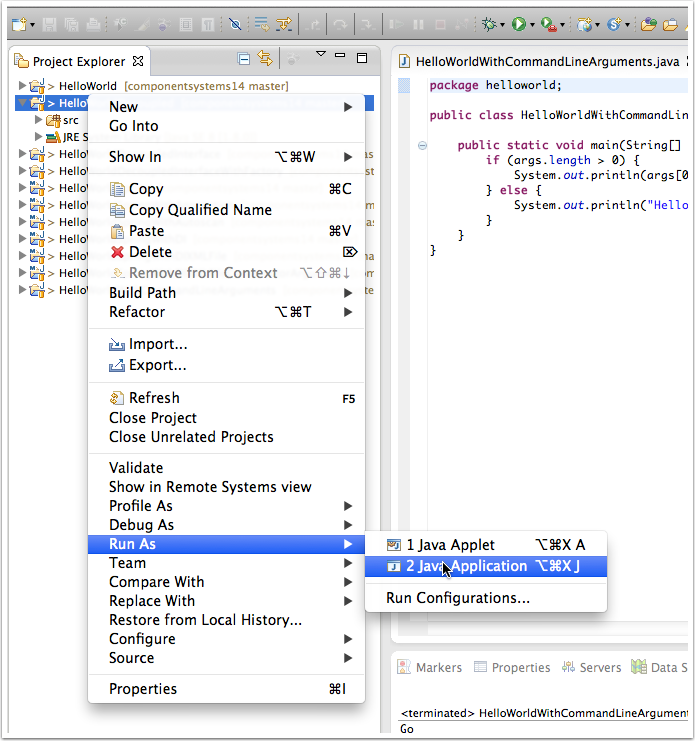
\includegraphics{images/HWD-run.png}

\item Observe that the text is displayed in the Console.

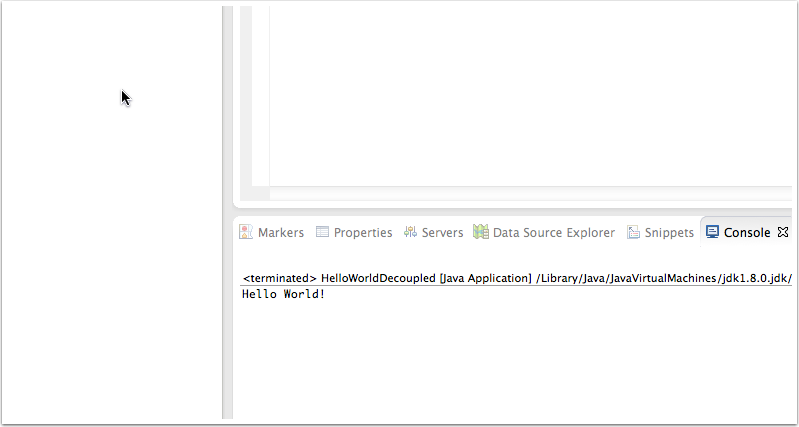
\includegraphics{images/HWD-run-result.png}

\end{enumerate}

\section{Build and Run \texttt{HelloWorldDecoupledInterface} sample application}

Now we are going to introduce Java interfaces so that the
message rendering logic does not get affected by the change in message
provider implementation.

\begin{enumerate}
\item Study the \texttt{HelloWorldDecoupledInterface} sample application

\bigskip

\VerbatimInput[frame=single,label=\fbox{\Large\emph{HelloWorldDecoupledInterface.java}}]{../../code/HelloWorldDecoupledInterface/src/helloworld/HelloWorldDecoupledInterface.java}

\bigskip

\VerbatimInput[frame=single,label=\fbox{\Large\emph{StandardOutMessageRenderer.java}}]{../../code/HelloWorldDecoupledInterface/src/helloworld/StandardOutMessageRenderer.java}

\bigskip

\VerbatimInput[frame=single,label=\fbox{\Large\emph{MessageRenderer.java}}]{../../code/HelloWorldDecoupledInterface/src/helloworld/MessageRenderer.java}

\bigskip

\VerbatimInput[frame=single,label=\fbox{\Large\emph{HelloWorldMessageProvider.java}}]{../../code/HelloWorldDecoupledInterface/src/helloworld/HelloWorldMessageProvider.java}

\bigskip

\VerbatimInput[frame=single,label=\fbox{\Large\emph{MessageProvider.java}}]{../../code/HelloWorldDecoupledInterface/src/helloworld/MessageProvider.java}
\bigskip

	\item Run \texttt{HelloWorldDecoupledInterface} sample application

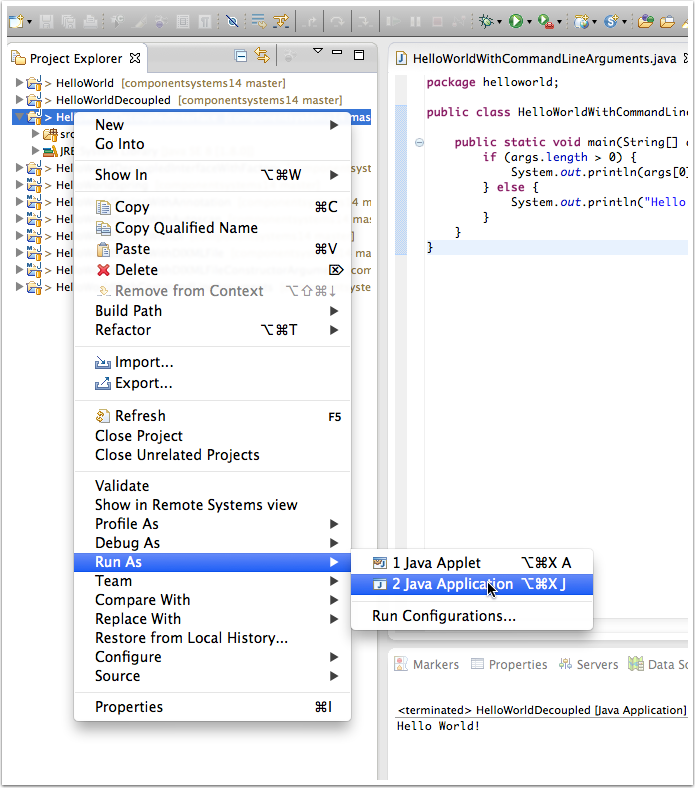
\includegraphics{images/HWDI.png}

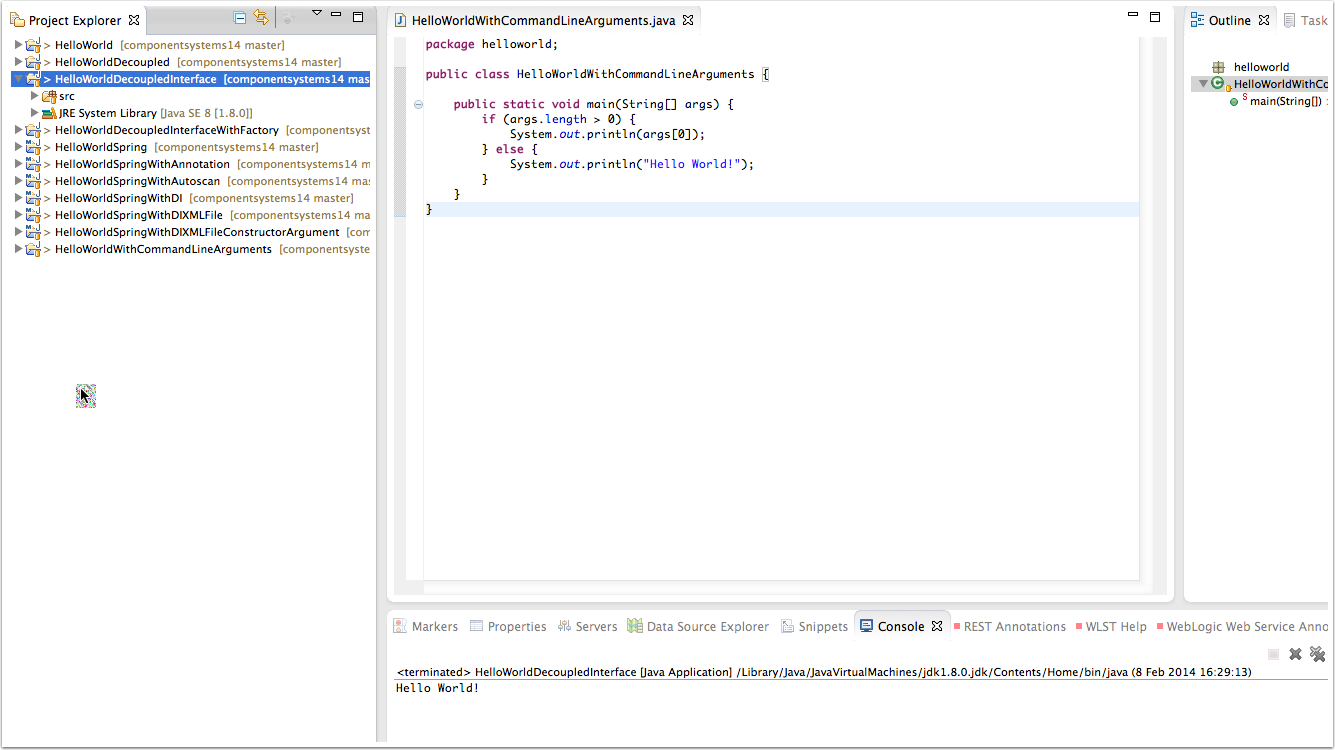
\includegraphics{images/HWDI-run.png}

\end{enumerate}

\section{Build and Run \texttt{HelloWorldDecoupledInterfaceWithFactory} sample application}

In this step, the properties file is used so that the message provider
implementation and the message renderer implementation can be replaced
simply by changing the properties file. 
So no change is required in the business logic code (launcher).

\begin{enumerate}
\item Study the \texttt{HelloWorldDecoupledInterface} sample application

\bigskip

\VerbatimInput[frame=single,label=\fbox{\Large\emph{HelloWorldDecoupledWithFactory.java}}]{../../code/HelloWorldDecoupledInterfaceWithFactory/src/helloworld/HelloWorldDecoupledWithFactory.java}

\bigskip

\VerbatimInput[frame=single,label=\fbox{\Large\emph{MessageSupportFactory.java}}]{../../code/HelloWorldDecoupledInterfaceWithFactory/src/helloworld/MessageSupportFactory.java}

\bigskip

\VerbatimInput[frame=single,label=\fbox{\Large\emph{bean.properties}}]{../../code/HelloWorldDecoupledInterfaceWithFactory/bean.properties}

\bigskip

\item Run \texttt{HelloWorldDecoupledInterfaceWithFactory} sample application

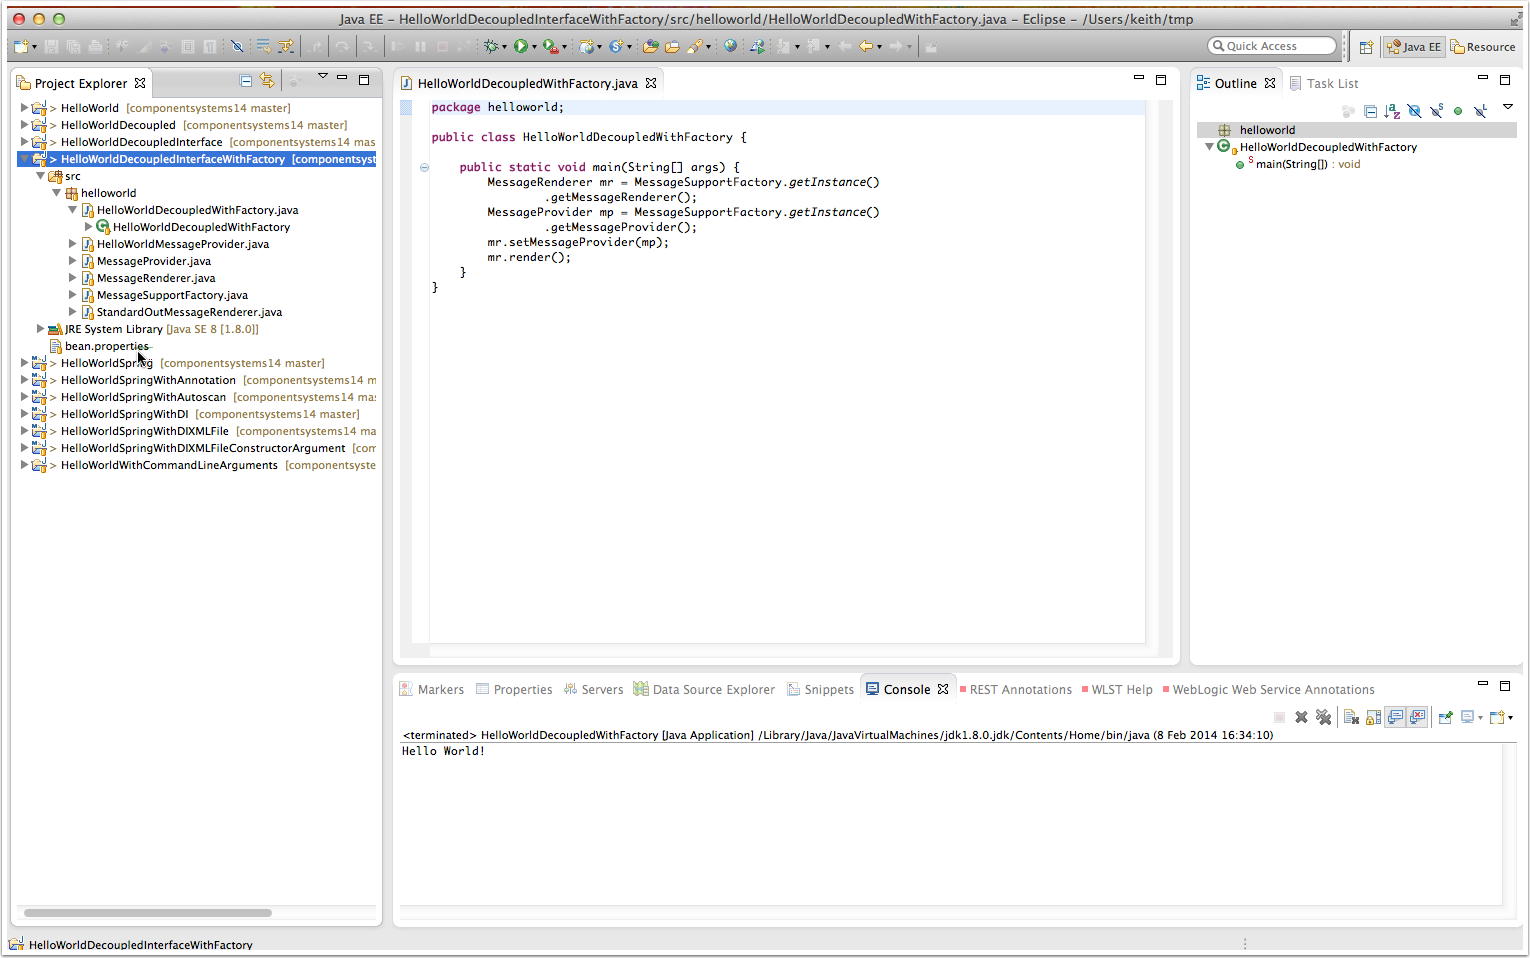
\includegraphics{images/HWDIWF---run.png}

\end{enumerate}

\section{Build and Run \texttt{HelloWorldSpring} sample application}

Now you are going to remove the need of your own \emph{glue code}
(\texttt{MessageSupportFactory}) and use the Spring provided factory class instead.

\begin{enumerate}
\item Study the \texttt{HelloWorldSpring} sample application

\bigskip

\VerbatimInput[frame=single,label=\fbox{\Large\emph{HelloWorldSpring.java}}]{../../code/HelloWorldSpring/src/main/java/helloworld/HelloWorldSpring.java}

\bigskip

\VerbatimInput[frame=single,label=\fbox{\Large\emph{beans.properties}}]{../../code/HelloWorldSpring/beans.properties}

\bigskip

\item Run \texttt{HelloWorldSpring} sample application
\end{enumerate}

\section{Build and Run \texttt{HelloWorldSpringWithDI} sample application}

In this step you are going to use the Spring framework Dependency Injection
(DI) mechanism.
The \texttt{main()} method now just obtains the \texttt{MessageRenderer} bean and
calls \texttt{render()}.
It does not have to obtain the \texttt{MessageProvider} bean and set
the \texttt{MessageProvider} property of the \texttt{MessageRenderer} bean itself because
the \emph{wiring} is performed through the Spring framework's Dependency
Injection mechanism.

\begin{enumerate}
\item Study the \texttt{HelloWorldSpringWithDI} sample application

\bigskip

\VerbatimInput[frame=single,label=\fbox{\Large\emph{HelloWorldSpringWithDI.java}}]{../../code/HelloWorldSpringWithDI/src/main/java/helloworld/HelloWorldSpringWithDI.java}

\bigskip

\VerbatimInput[frame=single,label=\fbox{\Large\emph{beans.properties}}]{../../code/HelloWorldSpringWithDI/beans.properties}

\bigskip

\item Run \texttt{HelloWorldSpringWithDI} sample application

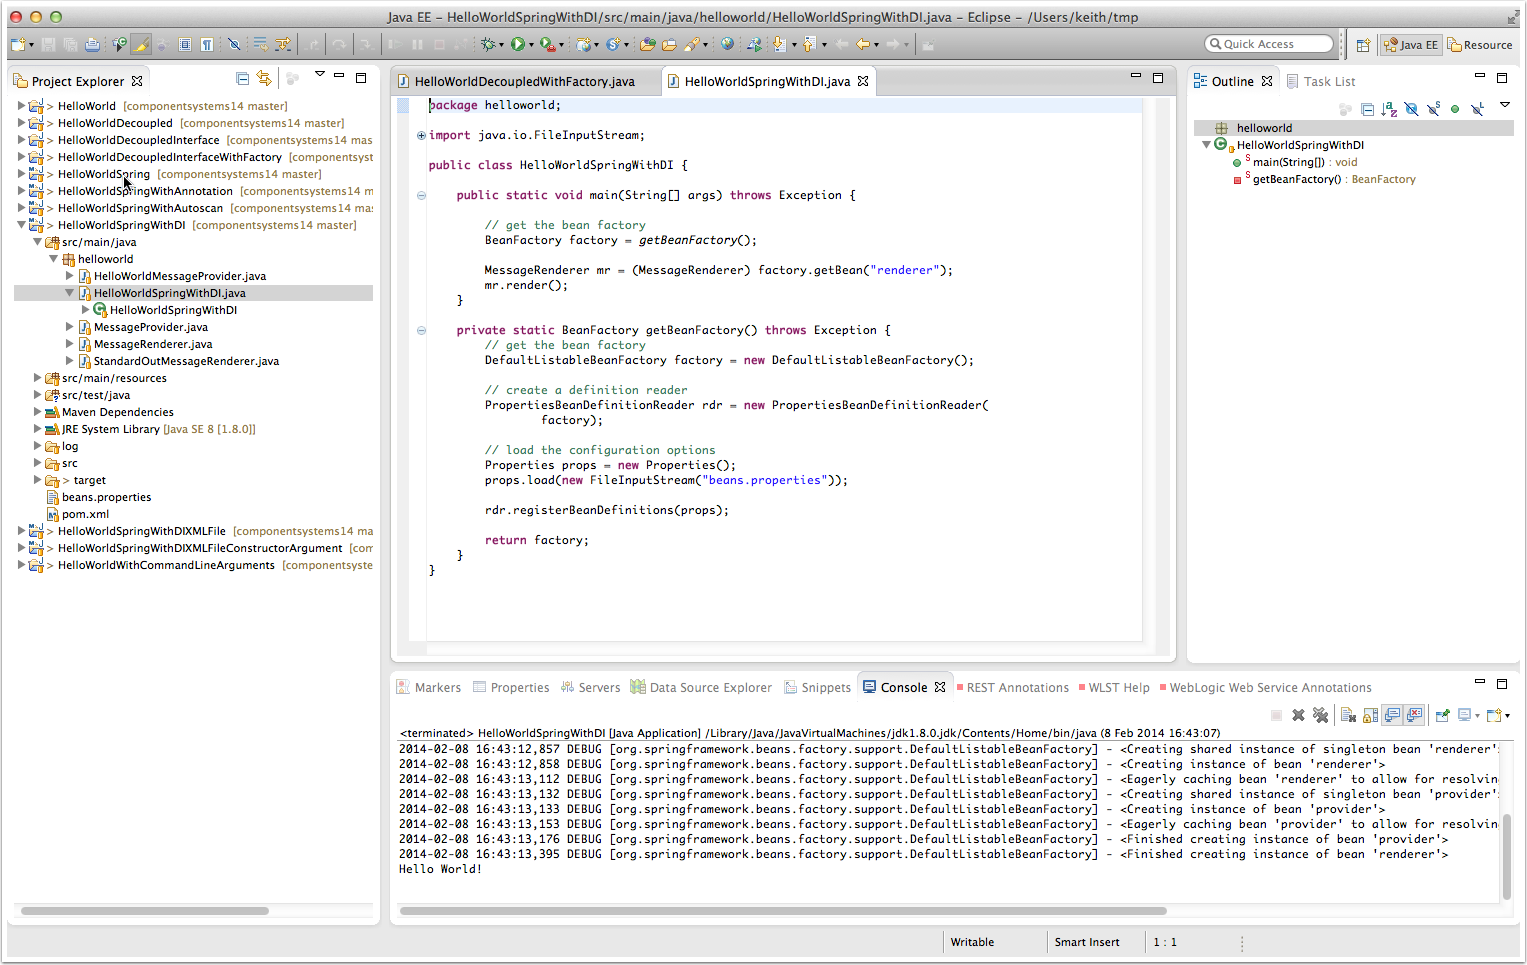
\includegraphics{images/HWSWDI---run.png}

\end{enumerate}

\section{Build and Run \texttt{HelloWorldSpringWithDIXMLFile} sample application}

In this step, you are going to use an XML file in which the wiring
requirements are specified.

\begin{enumerate}
	\item Study the \texttt{HelloWorldSpringWithDIXMLFile} sample application
\bigskip

\VerbatimInput[frame=single,label=\fbox{\Large\emph{HelloWorldSpringWithDIXMLFile.java}}]{../../code/HelloWorldSpringWithDIXMLFile/src/main/java/helloworld/HelloWorldSpringWithDIXMLFile.java}

\bigskip

%\VerbatimInput[frame=single,label=\fbox{\Large\emph{beans.xml}}]{../../code/HelloWorldSpringWithDIXMLFile/pom.xml}

	\item Run \texttt{HelloWorldSpringWithDIXMLFile} sample application
\end{enumerate}

\section{Build and Run \texttt{HelloWorldSpringWithDIXMLFileConstructorArgument} sample application}

In this step, you are going to change the wiring requirement using the constructor.

\begin{enumerate}
	\item Study the \texttt{HelloWorldSpringWithDIXMLFileConstructorArgument} sample application
\bigskip

\VerbatimInput[frame=single,label=\fbox{\Large\emph{HelloWorldSpringWithDIXMLFileConstructorArgument.java}}]{../../code/HelloWorldSpringWithDIXMLFileConstructorArgument/src/main/java/helloworld/HelloWorldSpringWithDIXMLFileConstructorArgument.java}

\bigskip

\VerbatimInput[frame=single,label=\fbox{\Large\emph{beans.xml}}]{../../code/HelloWorldSpringWithDIXMLFileConstructorArgument/src/main/resources/beans.xml}
\bigskip

\VerbatimInput[frame=single,label=\fbox{\Large\emph{ConfigurableMessageProvider.java}}]{../../code/HelloWorldSpringWithDIXMLFileConstructorArgument/src/main/java/helloworld/ConfigurableMessageProvider.java}

	\item Run \texttt{HelloWorldSpringWithDIXMLFileConstructorArgument} sample application
\end{enumerate}

\section{Build and Run \texttt{HelloWorldSpringWithAnnotation} sample application}

In this step, you are going to use Java annotations as the injection mechanism.

\begin{enumerate}
	\item Study the code
\bigskip

\VerbatimInput[frame=single,label=\fbox{\Large\emph{StandardOutMessageRenderer.java}}]{../../code/HelloWorldSpringWithDIXMLFileConstructorArgument/src/main/java/helloworld/StandardOutMessageRenderer.java}
\bigskip

\VerbatimInput[frame=single,label=\fbox{\Large\emph{beans.xml}}]{../../code/HelloWorldSpringWithDIXMLFileConstructorArgument/src/main/resources/beans.xml}
\bigskip

	\item Run \texttt{HelloWorldSpringWithAnnotation} sample application

\end{enumerate}

\section{Build and Run \texttt{HelloWorldSpringWithAutoscan} sample application}

In this step, you are going to use the \emph{autoscan} feature of Spring DI.

\begin{enumerate}
	\item Study the code

\VerbatimInput[frame=single,label=\fbox{\Large\emph{beans.xml}}]{../../code/HelloWorldSpringWithAutoscan/src/main/resources/beans.xml}
\bigskip

\VerbatimInput[frame=single,label=\fbox{\Large\emph{StandardOutMessageRenderer.java}}]{../../code/HelloWorldSpringWithAutoscan/src/main/java/helloworld/StandardOutMessageRenderer.java}
\bigskip

\VerbatimInput[frame=single,label=\fbox{\Large\emph{HelloWorldMessageProvider.java}}]{../../code/HelloWorldSpringWithAutoscan/src/main/java/helloworld/HelloWorldMessageProvider.java}

	\item Run \texttt{HelloWorldSpringWithAutoscan} sample application

\end{enumerate}

\end{document}